% Τεχνική αναφορά — μοντέλο προσομοίωσης και αποτελέσματα.
% Μεταγλώττιση: xelatex report.tex (δύο φορές)
\documentclass[11pt,a4paper]{article}

\usepackage{fontspec}
\usepackage{polyglossia}
\setmainlanguage{greek}
\setotherlanguage{english}
\setmainfont{Times New Roman}
\newfontfamily\greekfont{Times New Roman}
\setmonofont{Consolas}[Scale=0.85]

\usepackage[a4paper,left=2.4cm,right=2.4cm,top=2.4cm,bottom=2.4cm]{geometry}
\usepackage{amsmath,amssymb}
\usepackage{booktabs}
\usepackage{graphicx}
\usepackage{subcaption}
\graphicspath{{Results/}{Model/results/}}
\usepackage{caption}
\usepackage{enumitem}
\usepackage{fancyhdr}
\usepackage[hidelinks]{hyperref}
\usepackage{titlesec}

% Ανοχή στοίχισης για παραγράφους με άσπαστα μαθηματικά και μονάδες.
\emergencystretch=2em

\captionsetup{font=small,labelfont=bf}
\setlist{nosep,leftmargin=1.5em}
\titlespacing*{\section}{0pt}{2.4ex plus 1ex}{1.2ex}
\titlespacing*{\subsection}{0pt}{1.8ex plus 1ex}{0.8ex}
\titleformat{\section}{\large\bfseries}{\thesection.}{0.6em}{}
\titleformat{\subsection}{\normalsize\bfseries}{\thesubsection}{0.6em}{}

\pagestyle{fancy}
\fancyhf{}
\fancyhead[L]{\small Μοντέλο προσομοίωσης και αποτελέσματα}
\fancyhead[R]{\small\thepage}
\renewcommand{\headrulewidth}{0.4pt}

\begin{document}

\begin{center}
{\large\bfseries Διαχείριση πολλαπλής συνδεσιμότητας σε ολοκληρωμένα\\[2pt]
δορυφορικά–επίγεια δίκτυα 6G με χρήση μηχανικής μάθησης}\\[6pt]
{\normalsize Μέρος 1: μοντέλο προσομοίωσης, επαλήθευση και αποτελέσματα}\\[8pt]
{\small 30 Σεπτεμβρίου 2026}
\end{center}

\vspace{4pt}

\noindent\textbf{Περίληψη.} Η αναφορά περιγράφει το μοντέλο προσομοίωσης ενός
μεικτού επίγειου και δορυφορικού δικτύου, τη διαδικασία επαλήθευσής του και τα
αποτελέσματα μιας εκτέλεσης 202 διελεύσεων. Το μοντέλο υπολογίζει, ανά χρήστη
και ανά δευτερόλεπτο, τις απώλειες διάδοσης προς κάθε υποψήφιο κόμβο, τον λόγο
σήματος προς παρεμβολή και θόρυβο, τον κόμβο που επιλέγεται, τον ρυθμό που
επιτυγχάνεται και την κατανάλωση ισχύος. Η επιλογή κόμβου γίνεται με κανόνα
μέγιστου SINR, με υστέρηση και χρόνο επιβεβαίωσης κατά TS 38.331. Τα βασικά
αποτελέσματα είναι: σημείο ισοδυναμίας των δύο υποψηφίων στα 1\,473~m, ποσοστό
εξυπηρέτησης 60,67\% με διάστημα εμπιστοσύνης 1,67 εκατοστιαίων μονάδων, και
μέση διαφορά $+22{,}30 \pm 1{,}00$~Mbps της μεικτής πολιτικής έναντι της
αποκλειστικά επίγειας. Η υλοποίηση ελέγχεται με 52 αριθμητικούς ελέγχους και
182\,002 ελέγχους ανά βήμα προσομοίωσης.

\vspace{6pt}

\section{Εισαγωγή}

Αντικείμενο της εργασίας είναι η επιλογή κόμβου πρόσβασης σε δίκτυο που
συνδυάζει επίγειους σταθμούς βάσης και δορυφόρο χαμηλής τροχιάς. Το Μέρος~1,
που περιγράφεται εδώ, υλοποιεί την προσομοίωση και μια πολιτική επιλογής
αναφοράς. Το Μέρος~2 εκπαιδεύει μοντέλο μηχανικής μάθησης στα δεδομένα που
παράγει το Μέρος~1 και το συγκρίνει με την πολιτική αναφοράς.

Η προσομοίωση παράγει δύο αποτελέσματα. Το πρώτο είναι τα μετρικά μεγέθη του
δικτύου: χωρητικότητα, ποσοστό εξυπηρέτησης, κατανάλωση ενέργειας, πλήθος
μεταβολών κόμβου. Το δεύτερο είναι ένα επισημασμένο σύνολο δεδομένων, στο οποίο
κάθε γραμμή περιέχει τα χαρακτηριστικά που θα ήταν διαθέσιμα σε έναν αλγόριθμο
απόφασης και την απόφαση που λήφθηκε.

Το σύνολο του υπολογισμού γίνεται από ένα σενάριο, το \texttt{runSimulation.m}.
Μία εκτέλεση παράγει και τα μετρικά μεγέθη και το σύνολο δεδομένων.

\section{Μοντέλο συστήματος}

\subsection{Τοπολογία}

Το σενάριο περιλαμβάνει δύο επίγειους σταθμούς βάσης σε αστικό περιβάλλον και
έναν δορυφόρο σε κυκλική τροχιά ύψους 600~km. Το πλήθος των χρηστών ανά
διέλευση κληρώνεται από 3 έως 10 και οι θέσεις τους κατανέμονται
ομοιόμορφα κατά εμβαδόν σε δακτύλιο γύρω από έναν σταθμό αναφοράς. Οι χρήστες
κινούνται με σταθερή ταχύτητα 3~km/h και τυχαία κατεύθυνση, η οποία κληρώνεται
μία φορά ανά διέλευση [7, §8.4].

Οι ακτίνες των αρχικών θέσεων επιλέγονται ώστε καμία διαδρομή να μην μπορεί να
βγει από την περιοχή εγκυρότητας του μοντέλου διάδοσης κατά τη διάρκεια της
διέλευσης.

\begin{figure}[htbp]
\centering
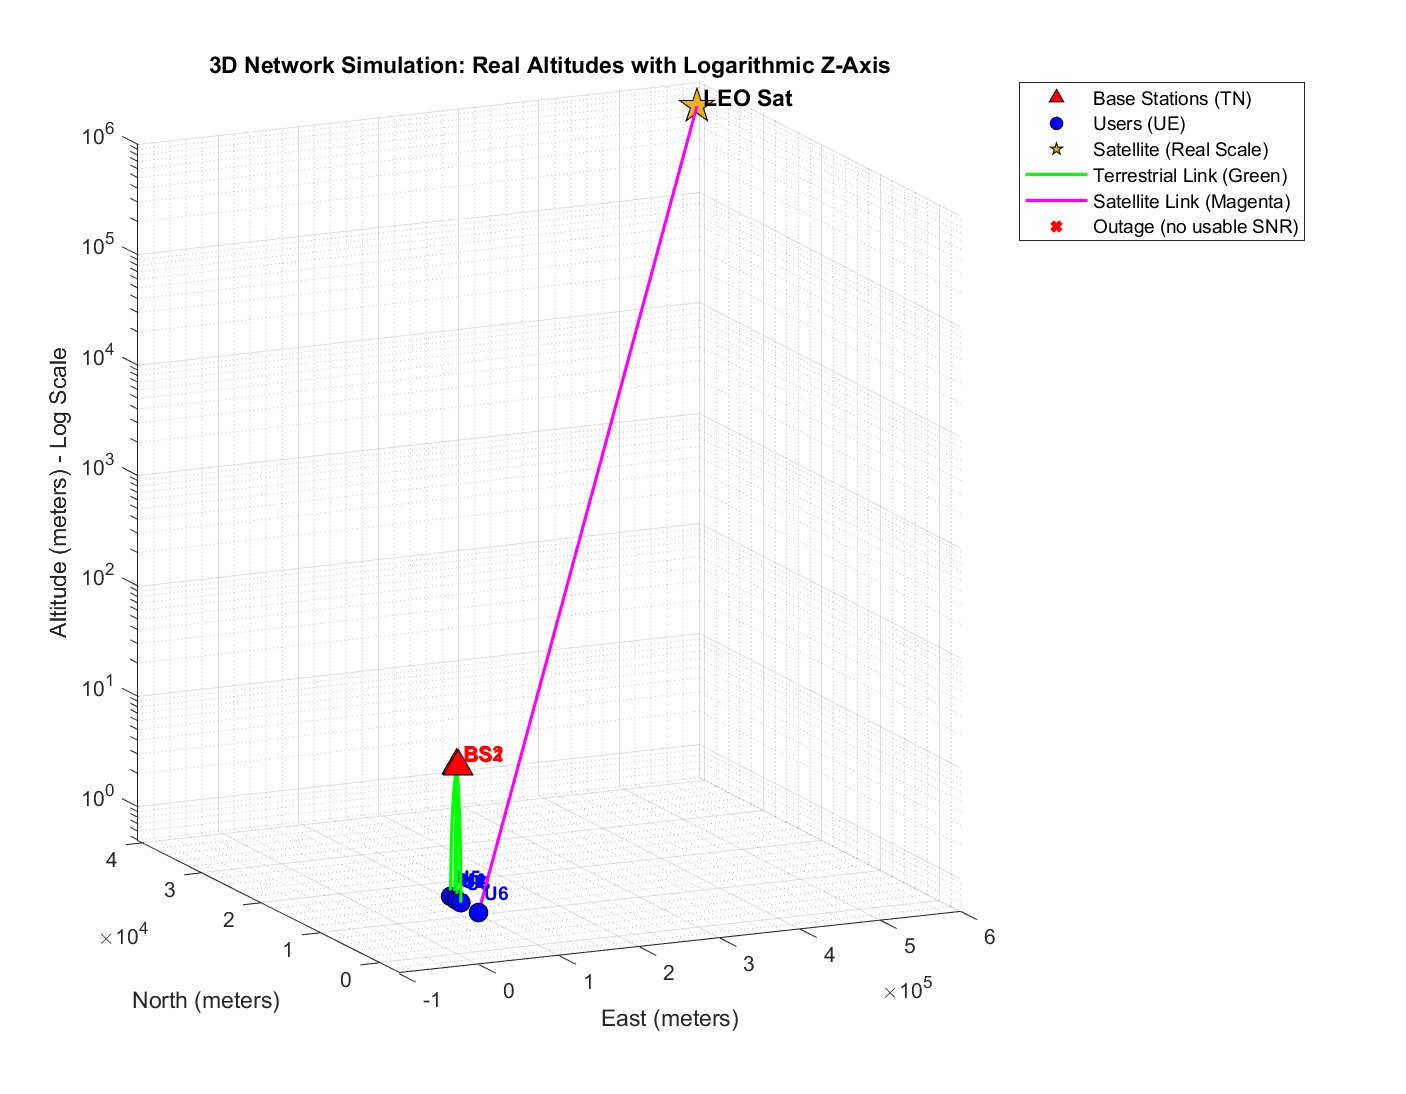
\includegraphics[width=\linewidth,trim=48 63 101 56,clip]{network_3d.png}
\caption{Στιγμιότυπο του σεναρίου. Ο κατακόρυφος άξονας είναι λογαριθμικός,
ώστε να απεικονίζονται μαζί ο σταθμός βάσης στα 25~m και ο δορυφόρος στα
600~km. Οι πράσινες γραμμές αντιστοιχούν σε επίγειες ζεύξεις και οι γραμμές
ματζέντα σε δορυφορικές. Οι ετικέτες παράγονται από τον κώδικα και είναι στα
αγγλικά.}
\label{fig:topology}
\end{figure}

\subsection{Διάδοση και κανάλι}

Ο Πίνακας~\ref{tab:model} συνοψίζει τα στοιχεία του μοντέλου και την πηγή
καθενός.

\begin{table}[htbp]
\centering\small
\caption{Στοιχεία του μοντέλου ζεύξης και πηγή τεκμηρίωσης.}
\label{tab:model}
\begin{tabular}{@{}p{4.2cm}p{5.9cm}p{5.1cm}@{}}
\toprule
Στοιχείο & Μοντελοποίηση & Πηγή \\
\midrule
Επίγειες απώλειες & UMa/UMi, με γεωδαισιακή οριζόντια απόσταση και φυσικά ύψη
κεραιών & [1], §7.4.1 \\
Περιοχή εγκυρότητας & $10$~m $\le d_{2D} \le 5$~km, ύψος τερματικού
$1{,}5$–$22{,}5$~m, συχνότητα $0{,}5$–$100$~GHz & [1], Πίν. 7.4.1-1 \\
Οπτική επαφή & Πιθανότητα εξαρτώμενη από την απόσταση, με χωρική συνέπεια
($d_{\mathrm{corr}} = 50$~m) & [1], §7.4.2 και §7.6.3.3 \\
Σκίαση & Λογαριθμοκανονική, με συσχέτιση AR(1) κατά τη μετακίνηση του χρήστη &
[1], §7.4.4 εξ. (7.4-5) \\
Επίγειες γρήγορες διαλείψεις & Rician με $K = 9$~dB σε οπτική επαφή, αλλιώς
Rayleigh & [1], Πίν. 7.5-6 \\
Δορυφορικές απώλειες & Ελεύθερος χώρος και αέρια απορρόφηση
$A_{\mathrm{zenith}}/\sin\varepsilon$ & [2], §6.6.4 εξ. (6.6-8)· [9] \\
Δορυφορικές διαλείψεις & Σκιασμένο Rician, με παραμέτρους από τη γωνία ανύψωσης
& [10], εξ. (19) και Πίν. III \\
EIRP επίγειο & $49 + 8 + 10\log_{10}(10) = 67$~dBm σύνθετο & [1], Πίν. 7.8-1 \\
EIRP δορυφορικό & Πυκνότητα $34$~dBW/MHz, δηλαδή $78{,}77$~dBm στα $30$~MHz &
[3], Πίν. 6.1.1.1-1 \\
Χωρητικότητα & Shannon, με ανώτατο όριο $5{,}5547$~bit/s/Hz & [5],
Πίν. 5.1.3.1-1 \\
\bottomrule
\end{tabular}
\end{table}

Δύο σημεία της υλοποίησης χρειάζονται διευκρίνιση.

Τα ύψη κεραιών εισάγονται στο μοντέλο ως φυσικά μεγέθη και δεν υπολογίζονται
από τοπικό καρτεσιανό σύστημα συντεταγμένων. Η καμπυλότητα της Γης κάνει το
δεύτερο να αποκλίνει με την απόσταση, και είχε οδηγήσει σε τιμές απωλειών της
τάξης των 755~dB σε προηγούμενη εκδοχή του κώδικα.

Η τιμή των 34~dBW/MHz του [3] είναι πυκνότητα EIRP και όχι ηλεκτρική ισχύς
ενισχυτή. Η ισχύς εισόδου στην κεραία προκύπτει ως
$\mathrm{EIRP} - G_{\mathrm{ant}} = 48{,}77$~dBm.

Στη δορυφορική ζεύξη δεν προστίθεται χωριστός όρος σκίασης. Η σκίαση
περιλαμβάνεται ήδη στο μοντέλο του σκιασμένου Rician, μέσω του πλάτους
Nakagami-$m$ της συνιστώσας οπτικής επαφής.

\subsection{Κεραία δορυφόρου}

Στον κώδικα χρησιμοποιείται σταθερό κέρδος 30~dBi, χωρίς εξάρτηση από τη γωνία
εκτός άξονα. Η επάρκεια της παραδοχής ελέγχθηκε αριθμητικά.

Το [2], §6.4.1 δίνει κανονικοποιημένο διάγραμμα κυκλικού ανοίγματος, με
$G(\theta) = 1$ επί του άξονα και $4\,|J_1(ka\sin\theta)/(ka\sin\theta)|^2$ για
$0 < |\theta| \le 90^\circ$. Επειδή το διάγραμμα είναι κανονικοποιημένο, τα
30~dBi αντιστοιχούν στην κορυφή και το διάγραμμα μόνο αφαιρεί· δεν προκύπτει
διπλή καταμέτρηση κέρδους.

Το σημείο $-3$~dB του διαγράμματος βρίσκεται στο $ka\sin\theta = 1{,}6163$.
Με ημιεύρος δέσμης $4{,}4127^\circ$ [3, Πίν. 6.1.1.1-1] προκύπτει $ka = 41{,}98$,
δηλαδή διάμετρος ανοίγματος 2,00~m. Για απόδοση ανοίγματος 55–60\% το κέρδος
που αντιστοιχεί σε αυτή τη διάμετρο είναι 29,9–30,2~dBi, σε συμφωνία με την
τιμή του ίδιου πίνακα.

Η περιοχή μελέτης ακτίνας 5~km υποτείνει γωνιακή ακτίνα το πολύ $0{,}48^\circ$,
έναντι εύρους δέσμης $4{,}41^\circ$. Η διαφορά κέρδους μεταξύ του κοντινότερου
και του πιο απομακρυσμένου χρήστη είναι επομένως το πολύ 0,13~dB, έναντι
τυπικής απόκλισης 5,14~dB των δορυφορικών διαλείψεων. Η παραδοχή του σταθερού
κέρδους ισχύει για αυτή την έκταση σεναρίου και δεν επεκτείνεται σε μεγαλύτερες
περιοχές ούτε στη συμπεριφορά κοντά στο όριο της δέσμης.

Η πολιτική στόχευσης είναι η Case~2 του [3, Πίν. 6.1.1.1-4], δηλαδή στόχευση
υπολογισμένη από γωνία ανύψωσης. Η εναλλακτική Case~1 (στόχευση στο ναδίρ) δεν
είναι ισοδύναμη: χρήστης σε ανύψωση $20^\circ$ θα βρισκόταν $59{,}2^\circ$
εκτός άξονα, δηλαδή σε εξασθένηση 46~dB.

\section{Κανόνας επιλογής κόμβου}

Ο κανόνας εφαρμόζεται ανά χρήστη και ανεξάρτητα για κάθε χρήστη. Αποτελείται από
τέσσερα σκέλη.

\subsection{Μέγιστο SINR}

Ο χρήστης συνδέεται στον κόμβο με το υψηλότερο SINR, μεταξύ των σταθμών βάσης
που βρίσκονται εντός της περιοχής εγκυρότητας και του δορυφόρου, εφόσον η
ανύψωση του τελευταίου είναι τουλάχιστον $20^\circ$. Η συνδεσιμότητα είναι
απλή: ένας κόμβος ή κανένας.

Στους επίγειους υποψηφίους υπολογίζεται παρεμβολή από τους υπόλοιπους σταθμούς:
\begin{equation}
\mathrm{SINR}_{u,b} \;=\; \frac{P_{u,b}}{N + \sum_{j\neq b} P_{u,j}} .
\end{equation}
Ο ορισμός προέρχεται από το [3, Πίν. 6.1.1.2-1 NOTE]. Η μοντελοποίηση της
παρεμβολής απαιτείται από το [7, §8.4 Πίν. 5~b) και §7.1]. Οι παραδοχές είναι
επαναχρησιμοποίηση συχνότητας 1 και συνεχής εκπομπή όλων των σταθμών,
ανεξάρτητα από το αν εξυπηρετούν χρήστες. Η δεύτερη παραδοχή διατηρεί το SINR
κάθε υποψηφίου ανεξάρτητο από την πολιτική επιλογής, κάτι που απαιτείται για τη
σύγκριση πολιτικών της Ενότητας~\ref{sec:policy}.

Στη δορυφορική ζεύξη ο όρος παρεμβολής είναι μηδενικός, οπότε το SINR ταυτίζεται
με τον λόγο σήματος προς θόρυβο.

\subsection{Υστέρηση και χρόνος επιβεβαίωσης}

Η αλλαγή κόμβου απαιτεί
\begin{equation}
\mathrm{SINR}_{\text{υποψηφίου}} - \mathrm{Hys} \;>\; \mathrm{SINR}_{\text{εξυπηρετούντος}}
\end{equation}
για $n = \lceil \mathrm{TTT}/\Delta t \rceil$ διαδοχικά βήματα. Η συνθήκη είναι
μεταφορά του γεγονότος A3 του [4, §5.5.4.4], με όλες τις μετατοπίσεις μηδενικές.
Τα επιτρεπτά σύνολα τιμών ορίζονται στο [4, §6.3.2]. Οι τιμές που
χρησιμοποιούνται, $\mathrm{Hys} = 3$~dB και $\mathrm{TTT} = 2560$~ms, προκύπτουν
από τη σάρωση της Ενότητας~\ref{sec:sweep}. Το κίνητρο για την υστέρηση είναι
το φαινόμενο εναλλαγής μεταξύ κόμβων, το οποίο το [3, §7.3.2.1.3] καταγράφει ως
πρόβλημα υψηλής προτεραιότητας για δορυφορικά δίκτυα.

Τρεις επιλογές υλοποίησης δηλώνονται. Η υστέρηση εφαρμόζεται σε όλους τους
υποψηφίους, άρα καλύπτει και τις εναλλαγές μεταξύ σταθμών βάσης. Εξυπηρετών
κόμβος του οποίου το SINR πέφτει κάτω από το κατώφλι διακοπής εγκαταλείπεται
άμεσα, χωρίς χρονομέτρηση. Κάθε πολιτική της σύγκρισης της
Ενότητας~\ref{sec:policy} διατηρεί χωριστή κατάσταση απόφασης.

Με μηδενικές τιμές και στις δύο παραμέτρους ο κανόνας ανάγεται στο απλό μέγιστο
SINR. Ελέγχθηκε ότι στην περίπτωση αυτή παράγεται ταυτόσημο σύνολο δεδομένων.

Με $\Delta t = 1$~s, 12 από τις 16 απαριθμημένες τιμές του \textsc{TimeToTrigger}
αντιστοιχούν σε λιγότερο από ένα βήμα και επομένως δεν διακρίνονται μεταξύ τους.
Διακριτά πλήθη βημάτων δίνουν μόνο οι τιμές 0, 1024, 2560 και 5120~ms.

\subsection{Κατώφλι διακοπής}

Αν το υψηλότερο SINR είναι κάτω από $-7{,}53$~dB, ο χρήστης δεν συνδέεται και
καταγράφεται σε κατάσταση διακοπής, με μηδενικό ρυθμό. Η κατανάλωση των κόμβων
συνεχίζει να προσμετράται στο σύνολο του δικτύου.

Η τιμή του κατωφλίου είναι το ισοδύναμο κατά Shannon SINR του χαμηλότερου
σχήματος διαμόρφωσης και κωδικοποίησης, MCS~0 (QPSK, $R = 120/1024$, δηλαδή
$0{,}2344$~bit/s/Hz) [5, Πίν. 5.1.3.1-2].

\subsection{Κατανομή πόρων και κριτήριο εξυπηρέτησης}

Το εύρος ζώνης του εξυπηρετούντος κόμβου μοιράζεται ισομερώς στους χρήστες του.
Η χωρητικότητα υπολογίζεται κατά Shannon και περιορίζεται στα
$5{,}5547$~bit/s/Hz, που αντιστοιχεί στο MCS~28 του πίνακα $\le$64QAM
[5, Πίν. 5.1.3.1-1].

Χωριστά από την επιλογή κόμβου, κάθε χρήστης ταξινομείται σε τρεις καταστάσεις
εξυπηρέτησης. Θεωρείται εξυπηρετούμενος αν ο ρυθμός του, κανονικοποιημένος στο
συνολικό εύρος ζώνης του κόμβου, φτάνει τα $0{,}3$~bit/s/Hz· αλλιώς
καταγράφεται ως κάτω του στόχου. Η τιμή είναι η απαίτηση του ITU-R M.2410 για
το 5ο εκατοστημόριο της φασματικής απόδοσης χρήστη [6, Πίν. 5.4.1.1.1-1], και η
κανονικοποίηση στο εύρος ζώνης καναλιού ορίζεται στο [6, §5.3].

Επειδή η κανονικοποίηση γίνεται στο συνολικό και όχι στο κατανεμημένο εύρος
ζώνης, το κριτήριο γίνεται αυστηρότερο όσο αυξάνεται το φορτίο του κόμβου:
απαιτείται $\mathrm{SE}_{\text{ζεύξης}} \ge 0{,}3\,L$ για $L$ χρήστες.

\section{Χρονική δομή και κριτήριο τερματισμού}

Η εκτέλεση είναι βρόχος πάνω σε διελεύσεις. Κάθε διέλευση αντιστοιχεί σε ένα
πέρασμα του δορυφόρου πάνω από την περιοχή και έχει διάρκεια 900~s, με κέντρο
τη μέγιστη προσέγγιση, ώστε και οι δύο διαβάσεις του ορίου ανύψωσης να
περιλαμβάνονται [3, Πίν. 4.2-3 NOTE 1].

Κάθε διέλευση αποτελεί ανεξάρτητη ρίψη κατά την έννοια του [7, §7.1]. Οι χρήστες
τοποθετούνται σε νέες θέσεις στην αρχή κάθε διέλευσης και η κατάσταση του
καναλιού δεν μεταφέρεται μεταξύ διελεύσεων. Η γεωμετρία μεταβάλλεται με
μετατόπιση του ορθού ανοδικού κόμβου της τροχιάς, ώστε οι διελεύσεις να
καλύπτουν το εύρος από οριακές έως σχεδόν κατακόρυφες. Η μέγιστη χρήσιμη
μετατόπιση υπολογίζεται αριθμητικά κατά την εκκίνηση.

Το βήμα είναι $\Delta t = 1$~s. Η τιμή προκύπτει από δύο ανεξάρτητους
περιορισμούς. Το [7, Παράρτημα 1 §5.3.2] θέτει ανώτατο όριο μετατόπισης
χρήστη 1~m ανά βήμα, που στα 3~km/h αντιστοιχεί σε 0,83~m. Το [3, §7.3.2.1.4]
δίνει ως ταχύτερη δορυφορική χρονική κλίμακα τα 6,61~s. Βήμα 5~s ικανοποιεί τον
πρώτο περιορισμό αλλά όχι τον δεύτερο.

Η συνολική διάρκεια δεν ορίζεται εκ των προτέρων. Ο βρόχος τερματίζεται όταν το
ημιεύρος του 95\% διαστήματος εμπιστοσύνης των παρακολουθούμενων μεγεθών,
υπολογισμένο μεταξύ διελεύσεων, πέσει κάτω από την ανοχή: 5\% σχετικό για
ρυθμούς και ενέργεια, 2 εκατοστιαίες μονάδες για ποσοστά. Το κριτήριο
προέρχεται από το [7, §7.1], το οποίο επεκτείνεται ρητά σε δορυφορικές
αξιολογήσεις από το [8, §8.2.4]. Οι πίνακες βαθμονόμησης του [3] δεν
περιλαμβάνουν πεδίο διάρκειας.

\section{Ενεργειακό μοντέλο}

Για τον σταθμό βάσης χρησιμοποιείται το γραμμικό μοντέλο EARTH [11, εξ. (1)],
\begin{equation}
P \;=\; N_{\mathrm{TRX}}\,\bigl(P_0 + \Delta_p\, P_{\mathrm{out}}\bigr),
\end{equation}
με τις τιμές αναφοράς για macro σταθμό: $P_0 = 130$~W, $\Delta_p = 4{,}7$,
$P_{\mathrm{sleep}} = 75$~W, $N_{\mathrm{TRX}} = 4$. Η ισχύς
$P_{\mathrm{out}}$ ορίζεται ανά αλυσίδα εκπομπής και το όριο εγκυρότητας του
μοντέλου, $P_{\max} = 20$~W [11, Πίν. 2], ελέγχεται κατά την εκτέλεση.

Για τον δορυφόρο χρησιμοποιείται γραμμικό μοντέλο ενισχυτή,
$P = P_{\mathrm{fix}} + P_{\mathrm{out}}/\eta_{\mathrm{PA}}$ με
$\eta_{\mathrm{PA}} = 0{,}4$ και $P_{\mathrm{fix}} = 0$. Η τιμή αυτή παραλείπει
την κατανάλωση της πλατφόρμας και συνιστά αισιόδοξη παραδοχή υπέρ του
δορυφορικού σκέλους.

Η ενέργεια ανά bit ορίζεται ως το πηλίκο της ισχύος του κόμβου ανά χρήστη προς
τον ρυθμό του χρήστη. Το φορτίο απλοποιείται αλγεβρικά:
$E = P/(B \cdot \mathrm{SE})$. Το μέγεθος είναι επομένως δείκτης απόδοσης
ζεύξης και δεν μεταβάλλεται με το πλήθος χρηστών ανά κόμβο. Η ιδιότητα
επαληθεύεται από χωριστό σενάριο.

Για τη σύγκριση των δύο τεχνολογιών καταγράφεται και το μέγεθος
\texttt{TotalPowerRf\_W}, το οποίο περιλαμβάνει μόνο το εξαρτώμενο από τον
ενισχυτή μέρος της κατανάλωσης, και στις δύο πλευρές.

\section{Επαλήθευση της υλοποίησης}

Η ορθότητα ελέγχεται σε τέσσερα ανεξάρτητα επίπεδα.

\paragraph{Αριθμητικοί έλεγχοι.} Σενάριο 52 ελέγχων σε οκτώ ομάδες συγκρίνει
κάθε τιμή του κώδικα με ανεξάρτητα υπολογισμένη κλειστή μορφή. Καλύπτονται οι
μετατροπές μονάδων και τα δύο EIRP, οι απώλειες ελεύθερου χώρου έναντι
$20\log_{10}(4\pi d/\lambda)$, ο θόρυβος $kTB$, η ταυτότητα
$\mathrm{SNR} = \mathrm{EIRP} - PL - N$, γνωστές συμπεριφορές (διπλασιασμός
απόστασης, $+6{,}021$~dB· διπλασιασμός εύρους ζώνης, $+3{,}010$~dB), η
διατήρηση του εύρους ζώνης κατά την κατανομή, το ισοζύγιο ισχύος, και τέσσερις
οριακές περιπτώσεις. Και οι 52 έλεγχοι περνούν, με μέγιστη απόκλιση
$4{,}8 \times 10^{-13}$.

Δύο από τους ελέγχους αφορούν ειδικά την παρεμβολή. Με έναν σταθμό βάσης,
αύξηση της ισχύος εκπομπής κατά 3~dB δίνει αύξηση του SINR ακριβώς κατά 3~dB.
Με δύο σταθμούς, η αύξηση είναι αυστηρά μικρότερη, επειδή αυξάνεται ταυτόχρονα
και η παρεμβολή.

\begin{figure}[htbp]
\centering
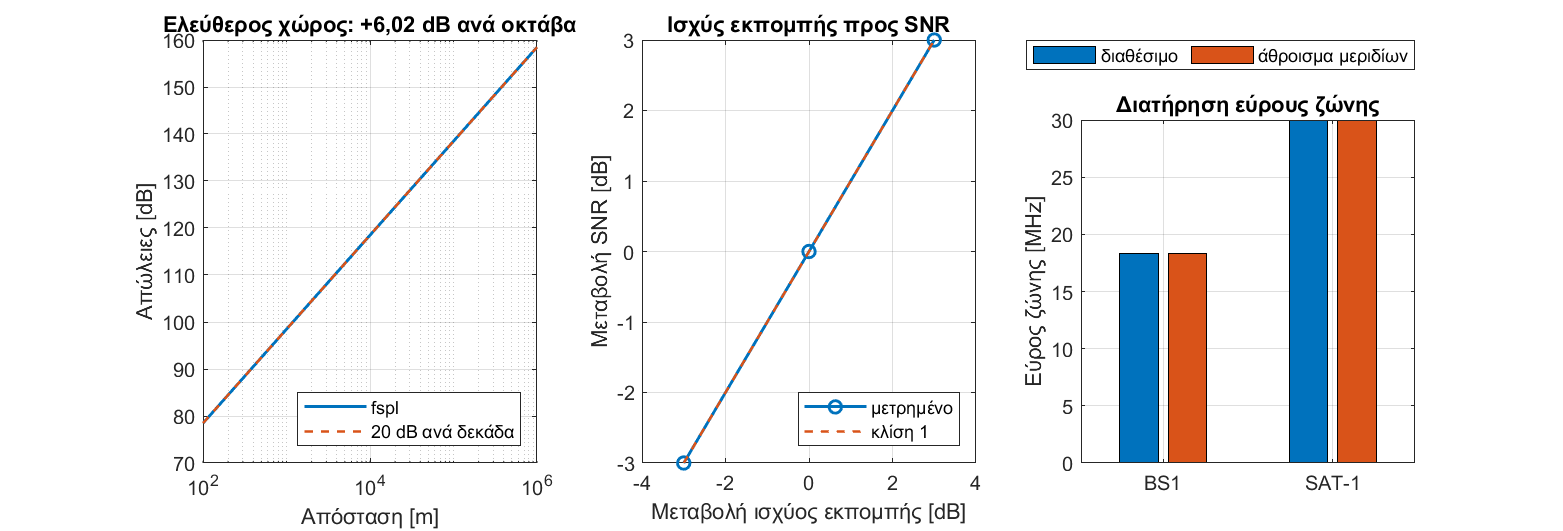
\includegraphics[width=\linewidth]{link_budget_validation.png}
\caption{Τρεις από τους 52 ελέγχους. Αριστερά: οι απώλειες ελεύθερου χώρου
ακολουθούν κλίση 20~dB ανά δεκάδα απόστασης. Κέντρο: μεταβολή της ισχύος
εκπομπής κατά $\pm 3$~dB δίνει μεταβολή SINR ακριβώς $\pm 3$~dB με έναν σταθμό
βάσης, αλλά αυστηρά μικρότερη με δύο, επειδή αυξάνεται ταυτόχρονα και η
παρεμβολή. Δεξιά: το άθροισμα των μεριδίων εύρους ζώνης των χρηστών ισούται με
το διαθέσιμο εύρος κάθε κόμβου.}
\label{fig:validation}
\end{figure}

\paragraph{Έλεγχοι ανά βήμα.} Σε κάθε βήμα κάθε διέλευσης, συνολικά
182\,002 φορές, ελέγχεται ότι το ύψος του τερματικού παραμένει 1,5~m, ότι οι
συντεταγμένες είναι πεπερασμένες και εντός ορίων, ότι κάθε χρήστης διαθέτει
τουλάχιστον μία επίγεια ζεύξη εντός της περιοχής εγκυρότητας, και ότι οι
γραμμές διακοπής φέρουν μηδενικό ρυθμό ενώ οι εξυπηρετούμενες φέρουν
πεπερασμένη χωρητικότητα και φορτίο τουλάχιστον 1. Παραβίαση οποιουδήποτε
ελέγχου τερματίζει την εκτέλεση και αναφέρει τη διέλευση, το βήμα και τον
χρήστη.

\paragraph{Έλεγχοι ουδετερότητας.} Κάθε αναδιάρθρωση του κώδικα ελέγχθηκε ως
προς το ότι δεν μεταβάλλει τα αριθμητικά αποτελέσματα, με σύγκριση όλων των
εξόδων σε τρεις γεωμετρίες και με σύγκριση της σύνοψης SHA-256 του συνόλου
δεδομένων πριν και μετά.

\paragraph{Σενάρια επαλήθευσης υπομοντέλων.} Δύο χωριστά σενάρια ελέγχουν τη
γεωμετρία των υψών κεραιών και το ενεργειακό μοντέλο. Και τα δύο τυπώνουν
ρητές γραμμές επιτυχίας ή αποτυχίας και τερματίζουν με σφάλμα στην πρώτη
αποτυχία.

\section{Αποτελέσματα}

\subsection{Σύγκλιση}

Το κριτήριο τερματισμού ικανοποιήθηκε στη διέλευση 202. Ο Πίνακας~\ref{tab:conv}
δίνει την κατάσταση των παρακολουθούμενων μεγεθών στο σημείο αυτό.

\begin{table}[htbp]
\centering\small
\caption{Παρακολουθούμενα μεγέθη στη διέλευση 202.}
\label{tab:conv}
\begin{tabular}{@{}lrrl@{}}
\toprule
Μέγεθος & Τιμή & Ημιεύρος ΔΕ 95\% & Ανοχή \\
\midrule
Μέση χωρητικότητα    & $15{,}04$~Mbps & $4{,}98\%$    & $5\%$ \\
Ποσοστό εξυπηρέτησης & $60{,}67\%$    & $1{,}67$ μον. & $2$ μον. \\
Ποσοστό δορυφορικών  & $25{,}84\%$    & $1{,}09$ μον. & $2$ μον. \\
Απόδοση bit/J (RF)   & $155\,711$     & $3{,}61\%$    & $5\%$ \\
\midrule
Μέσο SINR            & $3{,}78$~dB    & $4{,}84\%$    & εκτός κριτηρίου \\
\bottomrule
\end{tabular}
\end{table}

Το μέσο SINR καταγράφεται αλλά εξαιρείται από το κριτήριο τερματισμού. Είναι
μέσος όρος λογαριθμικού μεγέθους πάνω σε μεικτό πληθυσμό με εύρος δεκάδων dB
και συγκλίνει κατά μία τάξη μεγέθους πιο αργά από τα υπόλοιπα μεγέθη. Στην
εργασία το SINR αναφέρεται ως κατανομή.

Οι 202 διελεύσεις αντιστοιχούν σε 181\,800~s προσομοιωμένου χρόνου, δηλαδή
50,5 ώρες, και σε 234\,576 καταγεγραμμένες γραμμές, με μέσο όρο 6,42 χρηστών
ανά διέλευση.

\begin{figure}[htbp]
\centering
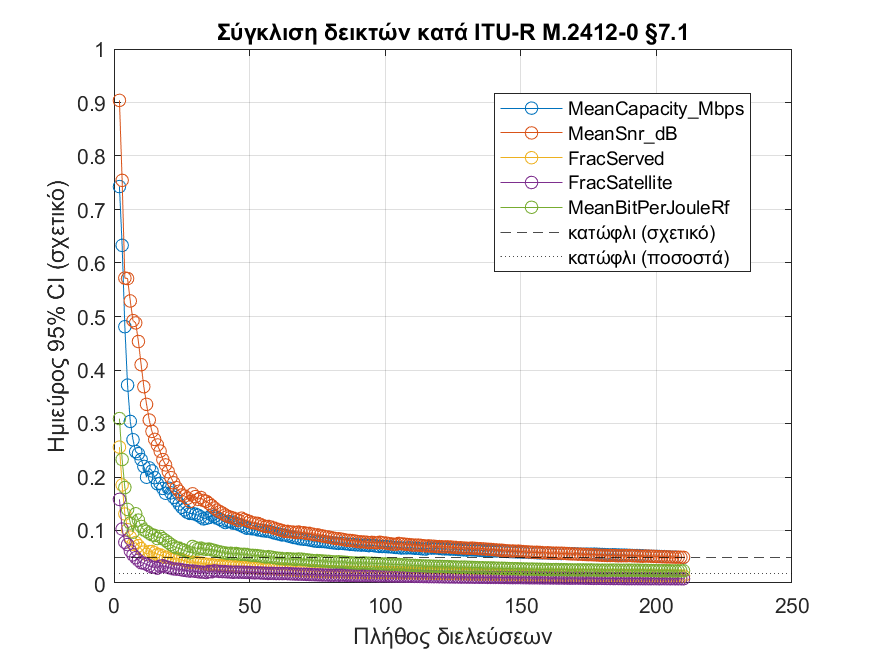
\includegraphics[width=0.68\linewidth]{convergence.png}
\caption{Ημιεύρος του 95\% διαστήματος εμπιστοσύνης, σε σχετικές μονάδες, ως
συνάρτηση του πλήθους διελεύσεων. Οι δύο οριζόντιες γραμμές είναι οι ανοχές
τερματισμού: 5\% για ρυθμούς και ενέργεια, 2 εκατοστιαίες μονάδες για ποσοστά.
Η εκτέλεση τερματίζεται στη διέλευση 202. Το μέσο SINR καταγράφεται αλλά δεν
συμμετέχει στο κριτήριο.}
\label{fig:convergence}
\end{figure}

\subsection{Κατανομή αποφάσεων και καταστάσεων εξυπηρέτησης}

\begin{table}[htbp]
\centering\small
\caption{Κατανομή των αποφάσεων επιλογής κόμβου και χαρακτηριστικά ανά τύπο
(διάμεσες τιμές).}
\label{tab:composition}
\begin{tabular}{@{}lrr@{\hspace{2.0em}}lrrrr@{}}
\toprule
Απόφαση & Γραμμές & \% & Τύπος & $C$ [Mbps] & SINR [dB] & $E$/bit [$\mu$J] & Φορτίο \\
\midrule
Επίγεια    & $153\,478$ & $65{,}43$ & Επίγειοι    & $6{,}86$  & $1{,}19$ & $40{,}16$ & $3$ \\
Δορυφορική & $60\,551$  & $25{,}81$ & Δορυφορικοί & $13{,}85$ & $7{,}91$ & $2{,}21$  & $6$ \\
Διακοπή    & $20\,547$  & $8{,}76$  &             &           &          &           &     \\
\bottomrule
\end{tabular}
\end{table}

Η κατανομή των καταστάσεων εξυπηρέτησης είναι 57,18\% εξυπηρετούμενοι, 34,06\%
κάτω του στόχου και 8,76\% σε διακοπή. Η σύγκριση με τη στήλη των αποφάσεων
δείχνει ότι πάνω από το ένα τρίτο των χρηστών συνδέεται σε κάποιον κόμβο χωρίς
να φτάνει το κατώφλι ποιότητας. Μέτρηση που βασιζόταν μόνο στη συνδεσιμότητα θα
έδινε ποσοστό επιτυχίας υψηλότερο κατά 34 μονάδες.

Οι δορυφορικοί χρήστες εμφανίζουν υψηλότερη διάμεσο χωρητικότητα παρά το
διπλάσιο φορτίο. Οι δύο αιτίες είναι το μεγαλύτερο εύρος ζώνης (30~MHz έναντι
18,36~MHz) και η απουσία παρεμβολής στη δορυφορική ζεύξη. Η δεύτερη είναι
συνέπεια της μοντελοποίησης μίας μόνο δέσμης και όχι ιδιότητα της τεχνολογίας.

\subsection{Σημείο τομής των δύο υποψηφίων}
\label{sec:crossover}

Για τις χρονικές στιγμές κατά τις οποίες ο δορυφόρος είναι ορατός, το ποσοστό
επιλογής του αυξάνεται με την απόσταση από τον πλησιέστερο σταθμό βάσης: από
31,7\% στη ζώνη 500–750~m έως 92\% πάνω από τα 4,5~km. Με γραμμική παρεμβολή
μεταξύ των δύο ζωνών εκατέρωθεν του 50\%, το σημείο στο οποίο οι δύο υποψήφιοι
είναι ισοδύναμοι βρίσκεται στα 1\,473~m.

Η μετάβαση είναι ομαλή, επειδή το επίγειο SINR δεν είναι ντετερμινιστική
συνάρτηση της απόστασης: η κατάσταση οπτικής επαφής, η σκίαση και η στάθμη της
παρεμβολής μετατοπίζουν το σημείο ισορροπίας ανά ζεύξη.

Η θέση του σημείου εξαρτάται από τη μοντελοποίηση της παρεμβολής. Χωρίς
παρεμβολή το ίδιο σημείο βρίσκεται στα 2\,206~m, δηλαδή η παρεμβολή το
μετατοπίζει κατά περίπου ένα τρίτο. Η ίδια αιτία εξηγεί γιατί η ακολουθία των
ποσοστών δεν είναι απολύτως μονότονη στις κοντινές ζώνες: όταν υπάρχει
παρεμβολή, η απόσταση από τον πλησιέστερο σταθμό δεν αρκεί για να προβλεφθεί η
ποιότητα της επίγειας ζεύξης, καθώς η στάθμη παρεμβολής εξαρτάται από τη θέση
του δεύτερου σταθμού.

\subsection{Ενέργεια}

\begin{table}[htbp]
\centering\small
\caption{Διάμεση ενέργεια ανά bit, με δύο εμβέλειες υποσυστημάτων.}
\label{tab:energy}
\begin{tabular}{@{}lrrr@{}}
\toprule
Εμβέλεια & Επίγειοι [$\mu$J] & Δορυφορικοί [$\mu$J] & Λόγος \\
\midrule
Πλήρης (όλα τα υποσυστήματα του σταθμού βάσης) & $40{,}16$ & $2{,}21$ & $18{,}2$ \\
Συμμετρική (μόνο ενισχυτής, και στις δύο πλευρές) & $16{,}78$ & $2{,}21$ & $7{,}6$ \\
\bottomrule
\end{tabular}
\end{table}

Ο λόγος μεταβάλλεται από 18,2 σε 7,6 ανάλογα με το ποια υποσυστήματα
περιλαμβάνονται στον υπολογισμό. Η πρώτη γραμμή συγκρίνει πλήρη σταθμό βάσης με
δορυφορικό ενισχυτή, ενώ η δεύτερη συγκρίνει ενισχυτή με ενισχυτή. Η σύγκριση
με ισοδύναμη εμβέλεια υποσυστημάτων είναι η δεύτερη. Και οι δύο τιμές
παραμένουν αισιόδοξες υπέρ του δορυφόρου, καθώς η κατανάλωση της πλατφόρμας δεν
μοντελοποιείται.

\subsection{Ευαισθησία στις παραμέτρους υστέρησης}
\label{sec:sweep}

Ο Πίνακας~\ref{tab:sweep} δίνει απόσπασμα σάρωσης δώδεκα ρυθμίσεων. Κάθε γραμμή
αντιστοιχεί σε πλήρη εκτέλεση με τις ίδιες υπόλοιπες παραμέτρους.

\begin{table}[htbp]
\centering\small
\caption{Μεταβολές κόμβου ανά χρήστη και ανά διέλευση, κατά προέλευση, και το
αντίστοιχο κόστος σε χωρητικότητα.}
\label{tab:sweep}
\begin{tabular}{@{}rrrrrrr@{}}
\toprule
Hys [dB] & TTT [ms] & Βήματα & Επίγ.–επίγ. & Επίγ.–δορ. & Σύνολο & $C$ [Mbps] \\
\midrule
$0$ & $0$    & $1$ & $136{,}8$ & $81{,}2$ & $218{,}0$ & $14{,}61$ \\
$3$ & $0$    & $1$ & $109{,}7$ & $52{,}8$ & $162{,}4$ & $14{,}31$ \\
$0$ & $2560$ & $3$ & $78{,}2$  & $16{,}6$ & $94{,}7$  & $13{,}12$ \\
$3$ & $2560$ & $3$ & $77{,}0$  & $13{,}4$ & $90{,}4$  & $13{,}03$ \\
$3$ & $5120$ & $6$ & $77{,}2$  & $11{,}7$ & $88{,}9$  & $13{,}14$ \\
\bottomrule
\end{tabular}
\end{table}

Προκύπτουν τρεις παρατηρήσεις.

Ο χρόνος επιβεβαίωσης έχει μεγαλύτερη επίδραση από την υστέρηση. Στα 2560~ms
και χωρίς υστέρηση, οι μεταβολές μειώνονται κατά 57\%. Η υστέρηση 3~dB χωρίς
χρόνο επιβεβαίωσης δίνει μείωση 26\%. Το αποτέλεσμα είναι συνεπές με τη φύση
του φαινομένου, καθώς οι εναλλαγές οφείλονται σε βραχύβιες ανατροπές της
σύγκρισης.

Το κόστος της επιλεγμένης ρύθμισης είναι περίπου 11\% στη χωρητικότητα και
5 εκατοστιαίες μονάδες στο ποσοστό εξυπηρέτησης. Το ποσοστό διακοπής είναι
9,94\% και στις δώδεκα ρυθμίσεις, κάτι που επαληθεύει την επιλογή υλοποίησης
ότι η υστέρηση δεν καθυστερεί την εγκατάλειψη κόμβου κάτω από το κατώφλι.

Καμία ρύθμιση δεν μειώνει τις μεταβολές μεταξύ σταθμών βάσης κάτω από περίπου
77 ανά χρήστη και διέλευση. Το κατώτατο αυτό όριο δεν οφείλεται σε ανεπαρκές
περιθώριο απόφασης, αλλά στο ότι οι γρήγορες διαλείψεις κληρώνονται ανεξάρτητα
σε κάθε βήμα, χωρίς χρονική συσχέτιση. Συνεπώς το πλήθος μεταβολών αποτελεί
άνω φράγμα και δεν αναφέρεται ως ρυθμός μεταπομπών. Αξιόπιστη εκτίμηση ρυθμού
μεταπομπών προϋποθέτει χρονικά συσχετισμένο μοντέλο διαλείψεων.

Σε ενδεικτική διέλευση, ο δορυφόρος ανατέλλει στα 216~s και δύει στα 564~s,
δηλαδή παράθυρο ορατότητας 348~s, με μέγιστη ανύψωση $55{,}9^\circ$. Το
συνολικό κόστος διακοπής από τις μεταπομπές είναι 343~ms σε 5\,406
βήματα-χρήστη, δηλαδή 0,0063\% του χρόνου.

\begin{figure}[htbp]
\centering
\begin{subfigure}{0.49\linewidth}
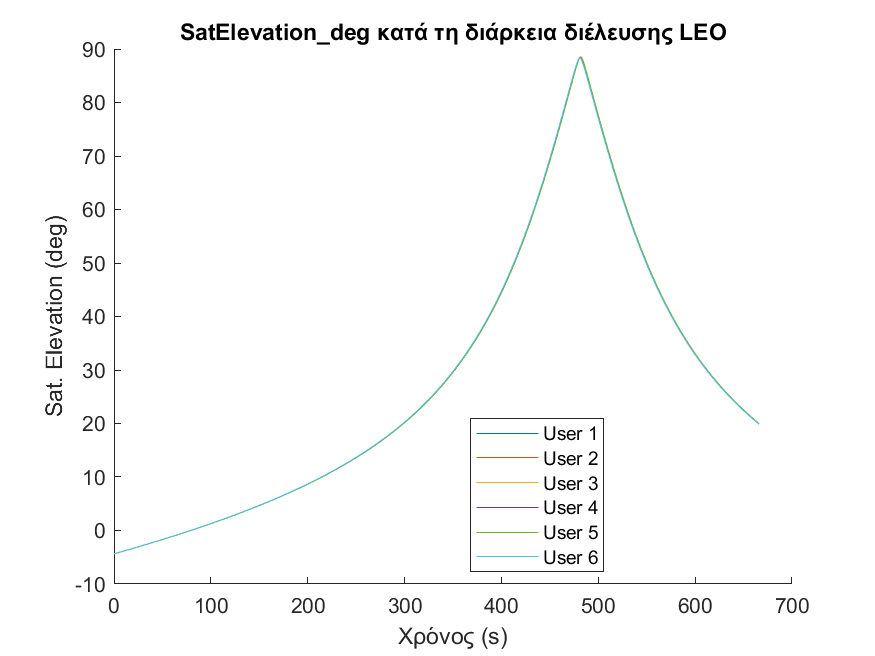
\includegraphics[width=\linewidth]{temporal_SatElevation_deg.png}
\end{subfigure}
\hfill
\begin{subfigure}{0.49\linewidth}
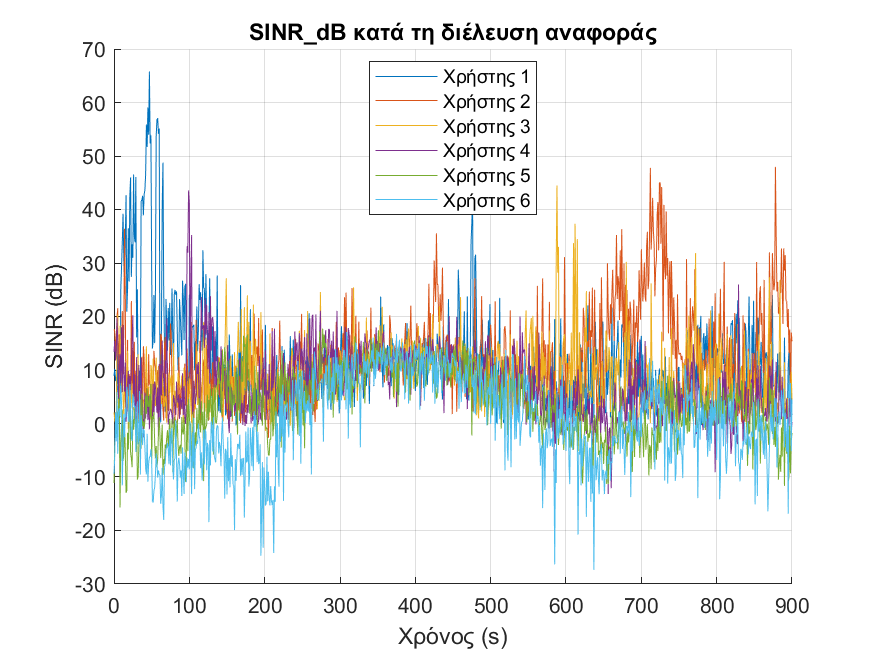
\includegraphics[width=\linewidth]{temporal_SINR_dB.png}
\end{subfigure}
\caption{Διέλευση αναφοράς. Αριστερά: γωνία ανύψωσης του δορυφόρου, σχεδιασμένη
μόνο για το διάστημα ορατότητας. Δεξιά: SINR των έξι χρηστών για ολόκληρο το
παράθυρο των 900~s. Η διακύμανση από βήμα σε βήμα οφείλεται στις γρήγορες
διαλείψεις, οι οποίες κληρώνονται ανεξάρτητα σε κάθε βήμα. Είναι η αιτία του
κατώτατου ορίου μεταβολών κόμβου που περιγράφηκε παραπάνω.}
\label{fig:refpass}
\end{figure}

\subsection{Σύγκριση πολιτικών σε ζεύγη}
\label{sec:policy}

Κάθε βήμα αποτιμάται τρεις φορές πάνω στην ίδια υλοποίηση του καναλιού: με τη
μεικτή πολιτική, με αποκλειστικά επίγεια επιλογή και με αποκλειστικά
δορυφορική. Η κατανομή πόρων υπολογίζεται εκ νέου για κάθε πολιτική, επειδή
μεταβάλλεται το φορτίο των κόμβων. Δεν εκτελούνται πρόσθετες τυχαίες κληρώσεις,
καθώς τα SINR και των δύο υποψηφίων υπολογίζονται ούτως ή άλλως για κάθε
χρήστη. Οι τρεις πολιτικές διαφέρουν μόνο ως προς την επιλογή.

Το στατιστικό είναι η διαφορά ανά κοινή διέλευση. Η επιλογή αυτή είναι
απαραίτητη επειδή οι χρήστες εντός μιας διέλευσης δεν είναι ανεξάρτητοι μεταξύ
τους.

\begin{table}[htbp]
\centering\small
\caption{Μέσες διαφορές ανά διέλευση της μεικτής πολιτικής έναντι των δύο
ακραίων, με 95\% διαστήματα εμπιστοσύνης (202 διελεύσεις).}
\label{tab:paired}
\begin{tabular}{@{}lrr@{}}
\toprule
Μέγεθος & Έναντι επίγειας & Έναντι δορυφορικής \\
\midrule
Συνολικός ρυθμός [Mbps]        & $+22{,}30 \pm 1{,}00$ & $+51{,}76 \pm 1{,}96$ \\
Ποσοστό εξυπηρέτησης [μονάδες] & $+10{,}63 \pm 0{,}57$ & $+38{,}51 \pm 1{,}27$ \\
Ποσοστό διακοπής [μονάδες]     & $-4{,}31 \pm 0{,}32$  & $-58{,}44 \pm 0{,}98$ \\
Απόδοση bit/J (RF)             & $+76\,497 \pm 5\,964$ & $-240\,158 \pm 5\,832$ \\
\midrule
Διελεύσεις με θετική διαφορά ρυθμού & $100\%$ & $100\%$ \\
\bottomrule
\end{tabular}
\end{table}

Η μεικτή πολιτική υπερέχει και των δύο ακραίων ως προς τον ρυθμό, το ποσοστό
εξυπηρέτησης και το ποσοστό διακοπής, σε όλες τις διελεύσεις. Υστερεί κατά
60,7\% σε ενεργειακή απόδοση έναντι της αποκλειστικά δορυφορικής. Η τελευταία
δεν ενεργοποιεί σταθμούς βάσης, αλλά αφήνει το 67,1\% των χρηστών σε διακοπή.
Οι δύο στήλες πρέπει να διαβάζονται μαζί.

Δύο επιφυλάξεις συνοδεύουν τα αποτελέσματα. Πρώτον, το ποσοστό των χρηστών κάτω
του στόχου δεν είναι μονότονο μεταξύ πολιτικών: πολιτική που αφήνει χρήστες σε
διακοπή εμφανίζει μικρότερο ποσοστό κάτω του στόχου, οπότε το μέγεθος αυτό
ερμηνεύεται μόνο μαζί με τα ποσοστά εξυπηρέτησης και διακοπής. Δεύτερον, η
σύγκριση αποτιμά τις αποφάσεις και όχι μια υλοποίηση: δεν περιλαμβάνει κόστος
σηματοδοσίας ούτε διακοπή μεταπομπής.

\subsubsection*{Πόσο από το πλεονέκτημα είναι απόφαση και πόσο φάσμα}

Η μεικτή πολιτική έχει στη διάθεσή της το άθροισμα των δύο ευρών ζώνης, ενώ
καθεμία από τις ακραίες μόνο το δικό της. Το ερώτημα αν το πλεονέκτημα
προέρχεται από την απόφαση ή απλώς από περισσότερο φάσμα χωρίζεται σε δύο μέρη
και έχει διαφορετική απάντηση σε καθένα.

\textbf{Οι μετρικές εξυπηρέτησης δεν επηρεάζονται.} Το κριτήριο της
Ενότητας~3.4 κανονικοποιείται στο εύρος ζώνης \emph{του κόμβου που
εξυπηρετεί}: ένας δορυφορικός χρήστης χρειάζεται $0{,}3 \times 30$~MHz, δηλαδή
$9$~Mbps, ενώ ένας επίγειος $0{,}3 \times 18{,}36 = 5{,}5$~Mbps. Το μεγαλύτερο
εύρος του δορυφόρου επιβάλλει αναλογικά αυστηρότερη απαίτηση, οπότε τα ποσοστά
εξυπηρέτησης, κάτω του στόχου και διακοπής είναι εξ ορισμού απαλλαγμένα από την
ασυμμετρία. Οι διαφορές $+10{,}63$ και $-4{,}31$ μονάδων του
Πίνακα~\ref{tab:paired} είναι επομένως αποτέλεσμα της απόφασης.

\textbf{Οι μετρικές ρυθμού επηρεάζονται, και το πρόσημο αντιστρέφεται.} Ο
δορυφόρος είναι ορατός κατά μέσο όρο στο $33{,}9\%$ του παραθύρου (εύρος
$10{,}6$–$40{,}9\%$), οπότε το φάσμα κάθε πολιτικής σταθμίζεται με τη
διαθεσιμότητά του.

\begin{table}[htbp]
\centering\small
\caption{Ρυθμαπόδοση ανά μονάδα πραγματικά διαθέσιμου φάσματος.}
\label{tab:spectral}
\begin{tabular}{@{}lrrr@{}}
\toprule
Πολιτική & Ρυθμός [Mbps] & Φάσμα $\times$ διαθεσ. [MHz] & bit/s/Hz \\
\midrule
Υπό εξέταση      & $78{,}14$ & $28{,}53$ & $2{,}739$ \\
Μόνο επίγεια     & $55{,}84$ & $18{,}36$ & $\mathbf{3{,}041}$ \\
Μόνο δορυφορική  & $26{,}37$ & $10{,}17$ & $2{,}594$ \\
\bottomrule
\end{tabular}
\end{table}

Ζευγαρωτά ανά διέλευση, η μεικτή πολιτική υστερεί της αποκλειστικά επίγειας
κατά $-0{,}301 \pm 0{,}028$~bit/s/Hz, με αρνητική διαφορά στο $94\%$ των
διελεύσεων. Το $+22{,}30$~Mbps είναι επομένως προίκα φάσματος και όχι ποιότητα
απόφασης.

Η αιτία είναι δομική. Οι δύο σταθμοί βάσης εκπέμπουν στα \emph{ίδια}
$18{,}36$~MHz, δηλαδή το επίγειο σκέλος διαθέτει χωρική επαναχρησιμοποίηση και
βγάζει διπλάσια χωρητικότητα από το ίδιο φάσμα. Ο δορυφόρος, με μία δέσμη, δεν
διαθέτει καμία: η οροφή του είναι $5{,}55$~bit/s/Hz έναντι $11{,}1$ του
επίγειου. Το αποτέλεσμα αυτό συνδέεται άμεσα με τον περιορισμό της
Ενότητας~\ref{sec:multibeam} — η διάταξη πολλαπλών δεσμών \emph{είναι} η
χωρική επαναχρησιμοποίηση του δορυφορικού σκέλους.

\begin{figure}[htbp]
\centering
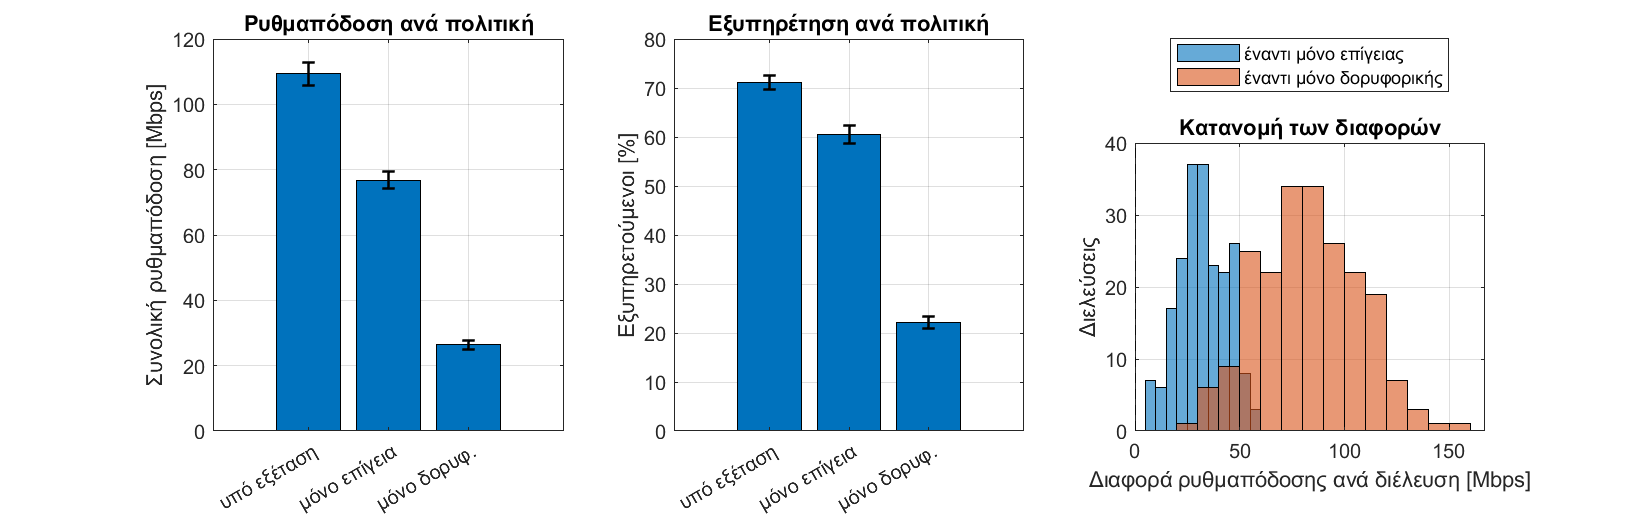
\includegraphics[width=\linewidth]{policy_comparison.png}
\caption{Αριστερά και κέντρο: συνολική ρυθμαπόδοση και ποσοστό εξυπηρέτησης ανά
πολιτική, με 95\% διαστήματα εμπιστοσύνης· η ένδειξη «υπό εξέταση» αντιστοιχεί
στη μεικτή πολιτική. Δεξιά: κατανομή της διαφοράς ρυθμαπόδοσης ανά διέλευση.
Και οι δύο κατανομές βρίσκονται εξ ολοκλήρου στα θετικά, δηλαδή η μεικτή
πολιτική υπερέχει σε κάθε μία από τις 202 διελεύσεις.}
\label{fig:policy}
\end{figure}

\subsection{Μοντέλα μηχανικής μάθησης}

Εκπαιδεύονται τέσσερις παραλλαγές, οι οποίες διαφέρουν μόνο ως προς την
πληροφορία που δίνεται στο μοντέλο. Και οι τέσσερις προβλέπουν δυαδικά τον
τύπο του εξυπηρετούντος κόμβου, χρησιμοποιούν μόνο χαρακτηριστικά επιπέδου
υποψηφίου και εξαιρούν τις γραμμές διακοπής. Ο διαχωρισμός σε σύνολο
εκπαίδευσης και ελέγχου γίνεται κατά διέλευση και όχι κατά γραμμή, επειδή κάθε
διέλευση είναι χρονοσειρά 900~s πάνω στην ίδια γεωμετρία.

Η συνολική ακρίβεια δεν είναι χρήσιμη μετρική εδώ, και αυτό πρέπει να
δηλωθεί πριν από κάθε αριθμό. Με υστέρηση η ετικέτα είναι έντονα
αυτοσυσχετισμένη: στο $88{,}96\%$ των διαδοχικών δειγμάτων ο τύπος κόμβου
μένει ίδιος. Ο κανόνας «πρόβλεψε ό,τι ίσχυε 5~s πριν», χωρίς κανένα μοντέλο και
κανένα χαρακτηριστικό, πιάνει $0{,}9468$ στο σύνολο ελέγχου — πάνω από δύο από
τις τρεις αρχικές παραλλαγές. Το σύνολο ελέγχου χωρίζεται επομένως σε
\textbf{σταθερές} στιγμές, όπου η ετικέτα ισούται με την προηγούμενη
($47\,402$ γραμμές, $88{,}5\%$), και σε \textbf{στιγμές αλλαγής}
($5\,883$, $11{,}0\%$). Σφάλμα στις πρώτες είναι \emph{ψευδής συναγερμός},
δηλαδή περιττή μεταπομπή· στις δεύτερες είναι \emph{χαμένη μετάβαση}.

\begin{table}[htbp]
\centering\small
\caption{Τυχαίο δάσος στο σύνολο ελέγχου (51 διελεύσεις, 53\,559 γραμμές·
εκπαίδευση σε 151 διελεύσεις, 160\,470 γραμμές), χωρισμένο σε σταθερές στιγμές
και στιγμές αλλαγής.}
\label{tab:ml}
\begin{tabular}{@{}lrrrrr@{}}
\toprule
Παραλλαγή & συνολικά & σταθερές & ψευδ. συναγ. & αλλαγές & χαμένες \\
\midrule
Ακριβές SINR      & $0{,}9502$ & $0{,}9616$ & $3{,}84\%$ & $\mathbf{0{,}8559}$ & $14{,}41\%$ \\
Θορυβώδες SINR    & $0{,}9386$ & $0{,}9532$ & $4{,}68\%$ & $\mathbf{0{,}8180}$ & $18{,}20\%$ \\
Μόνο γεωμετρία    & $0{,}9326$ & $0{,}9508$ & $4{,}92\%$ & $\mathbf{0{,}7831}$ & $21{,}69\%$ \\
Με μνήμη          & $0{,}9647$ & $0{,}9917$ & $\mathbf{0{,}83\%}$ & $0{,}7457$ & $25{,}43\%$ \\
\midrule
Εμμονή (χωρίς μοντέλο) & $0{,}9468$ & $1{,}0000$ & $0\%$ & $0{,}0000$ & $100\%$ \\
Πλειοψηφική κλάση      & $0{,}7074$ & — & — & — & — \\
\bottomrule
\end{tabular}
\end{table}

Η λογιστική παλινδρόμηση, με την ίδια σειρά, δίνει $0{,}9450$, $0{,}9379$,
$0{,}9327$ και $0{,}9583$ συνολικά, και $0{,}8295$, $0{,}8062$, $0{,}7829$,
$0{,}7149$ στις στιγμές αλλαγής.

Προκύπτουν τρία συμπεράσματα.

\textbf{Η ποιότητα της πληροφορίας μετράει, τετραπλάσια από ό,τι δείχνει η
συνολική ακρίβεια.} Οι τρεις αρχικές παραλλαγές απέχουν $1{,}8$ μονάδες
συνολικά αλλά $\mathbf{7{,}3}$ μονάδες στις στιγμές αλλαγής
($0{,}8559 \rightarrow 0{,}7831$), και το ποσοστό χαμένων μεταβάσεων πέφτει
κατά ένα τρίτο καθώς η είσοδος βελτιώνεται από τη γεωμετρία στο ακριβές SINR.

\textbf{Η μνήμη αγοράζει σταθερότητα, όχι ανίχνευση.} Με είσοδο τον
προηγούμενο εξυπηρετούντα κόμβο οι ψευδείς συναγερμοί πέφτουν κατά $4{,}6$
φορές, από $3{,}84\%$ σε $0{,}83\%$, αλλά η ανίχνευση των πραγματικών
μεταβάσεων χειροτερεύει από $0{,}8559$ σε $0{,}7457$. Ανά $1\,000$ δείγματα η
ανταλλαγή είναι περίπου $34 \rightarrow 7$ περιττές μεταπομπές έναντι
$16 \rightarrow 28$ χαμένες μεταβάσεις.

\textbf{Το μοντέλο με μνήμη έμαθε την ίδια την υστέρηση.} Αυτό είναι το
αναμενόμενο αποτέλεσμα της επίβλεψης σε ετικέτες που παρήγαγε μια πολιτική
υστέρησης, και ταυτόχρονα η οροφή: μοντέλο που μιμείται τις αποφάσεις μιας
πολιτικής δεν μπορεί να την ξεπεράσει. Για υπέρβαση απαιτείται διαφορετικός
στόχος — ρυθμαπόδοση, ενέργεια ή κόστος διακοπής — αντί για συμφωνία με τις
ετικέτες της.

Ο στιγμιαίος κανόνας μέγιστου SINR συμφωνεί με την καταγεγραμμένη απόφαση σε
219\,621 από 234\,576 γραμμές, δηλαδή $93{,}62\%$· οι $14\,955$ διαφωνίες
μετρούν πόσο συχνά η υστέρηση διατήρησε τον χρήστη σε κόμβο που δεν ήταν ο
στιγμιαία καλύτερος. Η ετικέτα έπαψε επομένως να είναι ντετερμινιστική
συνάρτηση των χαρακτηριστικών. Σημειώνεται τέλος ότι το χαρακτηριστικό του
χρόνου παραμονής αποδείχθηκε άχρηστο (σημαντικότητα μετάθεσης $0{,}0002$,
τελευταίο από έντεκα): με δειγματοληψία $5$~s δεν μπορεί να διακρίνει παράθυρο
επιβεβαίωσης $2560$~ms.

Ο κανόνας με μνήμη δεν μπορεί να αναπαραχθεί από τις δημοσιευμένες στήλες του
συνόλου δεδομένων, επειδή αυτό είναι δειγματοληπτημένο ανά 5~s και η ταυτότητα
του ανταγωνιστικού κόμβου δεν καταγράφεται όταν εξυπηρετεί ο δορυφόρος.

Ως προς τη σημαντικότητα χαρακτηριστικών, η μετάθεση επί του συνόλου ελέγχου
κατατάσσει πρώτες τις δορυφορικές απώλειες διάδοσης (0,133) και το δορυφορικό
SINR (0,077). Η σημαντικότητα της απόστασης από τον σταθμό βάσης μειώθηκε από
0,178 σε 0,073 με την εισαγωγή της παρεμβολής. Το εύρημα συμφωνεί με τη μη
μονοτονία των ποσοστών στις κοντινές ζώνες απόστασης
(Ενότητα~\ref{sec:crossover}).

\begin{figure}[htbp]
\centering
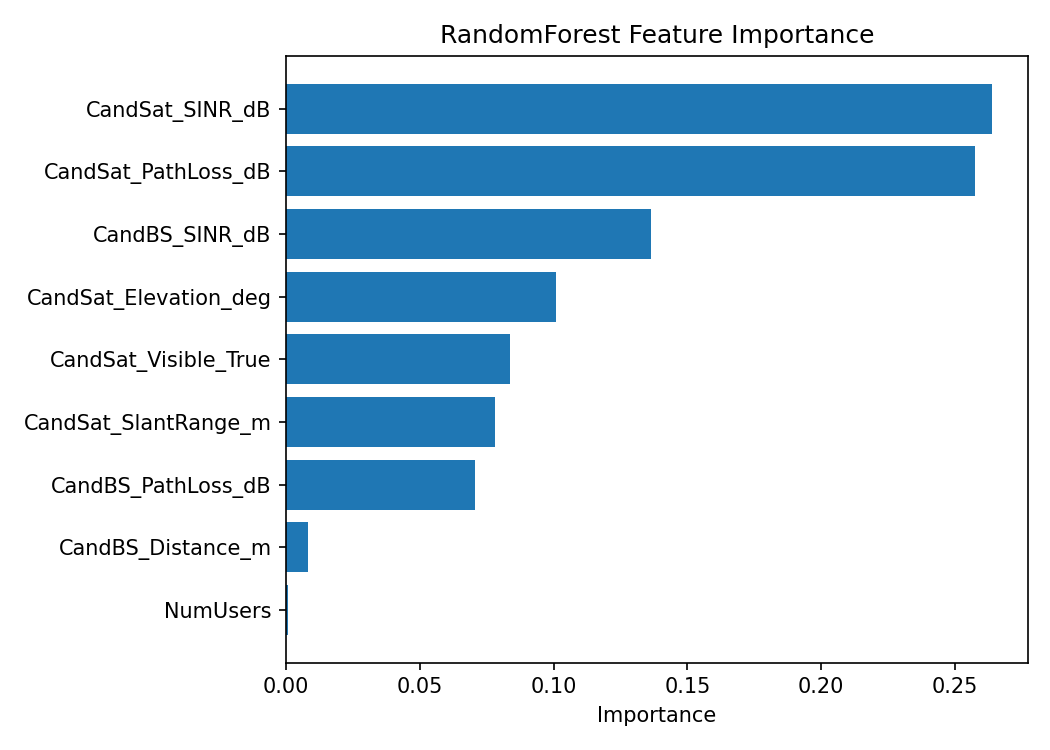
\includegraphics[width=0.66\linewidth]{feature_importance_RandomForest.png}
\caption{Σημαντικότητα χαρακτηριστικών κατά ακαθαρσία, για το τυχαίο δάσος της
παραλλαγής ακριβούς SINR. Οι τιμές διαφέρουν από αυτές της μετάθεσης που
αναφέρονται στο κείμενο, επειδή πρόκειται για διαφορετικό μέτρο: η ακαθαρσία
υπολογίζεται κατά την εκπαίδευση, ενώ η μετάθεση επί του συνόλου ελέγχου. Η
κατάταξη των χαρακτηριστικών είναι παρόμοια και στα δύο μέτρα.}
\label{fig:importance}
\end{figure}

\section{Περιορισμοί}

\begin{itemize}
\item Το πλήθος μεταβολών κόμβου αποτελεί άνω φράγμα και όχι ρυθμό μεταπομπών,
επειδή οι γρήγορες διαλείψεις κληρώνονται ανεξάρτητα σε κάθε βήμα.
\item Η παρεμβολή υποεκτιμάται, οπότε το SINR αποτελεί άνω φράγμα. Οι αιτίες
είναι δύο: το σενάριο περιλαμβάνει δύο μόνο σταθμούς βάσης, έναντι των 19
θέσεων με 3 τομείς που προβλέπει το [7, §8.3]· και σταθμός εκτός της περιοχής
εγκυρότητας του μοντέλου δεν προσμετράται ως παρεμβολέας, καθώς οι απώλειές του
δεν υπολογίζονται χωρίς παραβίαση του ορίου εγκυρότητας.
\item Η σύγκριση πολιτικών αποτιμά αποφάσεις και όχι υλοποίηση. Επιπλέον, η
μεικτή πολιτική διαθέτει το άθροισμα των δύο ευρών ζώνης (48,36~MHz έναντι
18,36 ή 30 χωριστά), οπότε μέρος του πλεονεκτήματός της οφείλεται στο διαθέσιμο
φάσμα.
\item Η σύγκριση κατανάλωσης εξαρτάται από την εμβέλεια των υποσυστημάτων και
είναι αισιόδοξη υπέρ του δορυφόρου, λόγω της παραδοχής $P_{\mathrm{fix}} = 0$.
\item Μοντελοποιείται μία δορυφορική δέσμη, οπότε δεν υπάρχει παρεμβολή
μεταξύ δεσμών. Είναι ο σημαντικότερος περιορισμός και ποσοτικοποιείται στην
Ενότητα~\ref{sec:multibeam}.
\item Το μοντέλο επίπεδων διαλείψεων εφαρμόζεται σε εύρη 20 και 30~MHz, ενώ το
[2, §6.7] θέτει ως προϋπόθεση εύρος έως 5~MHz. Η απόκλιση δηλώνεται και
χρειάζεται τεκμηρίωση ως προς τη διασπορά καθυστέρησης.
\item Δεν μοντελοποιούνται βροχή, νέφωση και ιονοσφαιρικός σπινθηρισμός. Η
επίδρασή τους στη ζώνη S είναι χαμηλή κατά το [2, §6.6.5], αλλά δεν έχει
ποσοτικοποιηθεί εδώ.
\end{itemize}

\subsection{Πολλαπλές δέσμες: πόσο κοστίζει ο περιορισμός}
\label{sec:multibeam}

Η μοντελοποίηση μίας δέσμης δεν είναι σφάλμα: το [3] ορίζει τις δορυφορικές
παραμέτρους — εύρος ζώνης, κέρδος, πυκνότητα EIRP — \emph{ανά δέσμη}, οπότε
μία δέσμη με παραμέτρους μίας δέσμης είναι εσωτερικά συνεπής διαμόρφωση, και η
διάταξη των 19 δεσμών ανήκει στη βαθμονόμηση πλήρους προσομοίωσης συστήματος.
Το κενό αφορά το εύρος του μοντέλου, όχι την ορθότητά του. Επειδή όμως δεν
είναι αμελητέο, δίνεται εδώ μετρημένο αντί απλώς δηλωμένο.

Ο Πίν. 6.1.1.1-4 του [3] ορίζει την απόσταση γειτονικών δεσμών στο επίπεδο UV
ως $\mathrm{ABS} = \sqrt{3}\,\sin(\mathrm{HPBW}/2)$. Με το ημιεύρος δέσμης
$4{,}4127^\circ$ προκύπτει γειτονική δέσμη $3{,}82^\circ$ εκτός άξονα, και με
το κανονικοποιημένο διάγραμμα του [2, §6.4.1] η συνεισφορά κάθε γειτονικής
δέσμης είναι $-10{,}7$~dB. Αξίζει να σημειωθεί ότι το γινόμενο
$ka \cdot \mathrm{ABS} = 2{,}7995$ είναι ανεξάρτητο του $ka$: η εξασθένηση
προς τη γειτονική δέσμη είναι ιδιότητα της διάταξης και όχι της κεραίας.
Αθροίζοντας το εξαγωνικό πλέγμα των 19 δεσμών, ο λόγος παρεμβολής προς σήμα
είναι $-1{,}3$~dB με συντελεστή επαναχρησιμοποίησης 1 και $-9{,}0$~dB με
συντελεστή 3. Το πρότυπο δίνει και τους δύο ως επιλογή.

Εφαρμόζοντας τα δύο αυτά επίπεδα παρεμβολής στα υπάρχοντα δεδομένα:

\begin{table}[htbp]
\centering\small
\caption{Εκτίμηση της επίδρασης της παρεμβολής μεταξύ δεσμών, με εφαρμογή του
υπολογισμένου λόγου $I/C$ στα αποτελέσματα της τρέχουσας εκτέλεσης.}
\label{tab:multibeam}
\begin{tabular}{@{}lrrr@{}}
\toprule
 & μία δέσμη & επαναχρ. 3 & επαναχρ. 1 \\
\midrule
Διάμεσο δορυφορικό SINR [dB] & $6{,}84$ & $4{,}78$ & $0{,}23$ \\
Δορυφορικό ποσοστό [\%]      & $24{,}76$ & $22{,}53$ & $15{,}29$ \\
\textbf{Σημείο τομής [m]}    & $\mathbf{1\,474}$ & $\mathbf{2\,080}$ & $\mathbf{3\,014}$ \\
Ποσοστό διακοπής [\%]        & $8{,}76$ & $8{,}76$ & $8{,}78$ \\
\bottomrule
\end{tabular}
\end{table}

Τρία πράγματα προκύπτουν. \textbf{Το ποσοστό διακοπής δεν μεταβάλλεται
καθόλου}: όταν υποβαθμίζεται ο δορυφόρος ο χρήστης πέφτει στο επίγειο σκέλος,
και ο δορυφόρος σπάνια είναι ο μόνος αξιοποιήσιμος υποψήφιος. \textbf{Το
δορυφορικό ποσοστό μεταβάλλεται λίγο}, κατά $2{,}2$ μονάδες με επαναχρησιμοποίηση
3, δηλαδή περίπου δύο πλάτη του διαστήματος εμπιστοσύνης του μεγέθους.
\textbf{Το σημείο τομής μεταβάλλεται πολύ}, κατά $+41\%$.

Το τελευταίο αξίζει έμφαση γιατί το σημείο τομής είναι το πρώτο ερευνητικό
ερώτημα. Η παρεμβολή μεταξύ επίγειων σταθμών το μετακίνησε από $2\,206$ σε
$1\,468$~m· η παρεμβολή μεταξύ δεσμών θα το επανέφερε στα $2\,080$~m. Πρόκειται
για δύο φαινόμενα αντίθετης φοράς και συγκρίσιμου μεγέθους, από τα οποία
μοντελοποιείται μόνο το ένα. Η τιμή των $1\,473$~m δεν είναι επομένως
εσφαλμένη, αλλά \emph{υπό όρους}: ισχύει για επίγειο σκέλος με παρεμβολή και
δορυφορικό με μία δέσμη, και η μεροληψία έχει γνωστή φορά — το τοποθετεί πιο
κοντά στον σταθμό βάσης απ' ό,τι θα ήταν.

Η εκτίμηση αυτή χρησιμοποιεί τον στιγμιαίο κανόνα επιλογής αντί του πλήρους με
υστέρηση, οι οποίοι συμφωνούν στο $93{,}62\%$ των γραμμών, και εφαρμόζει ενιαίο
λόγο $I/C$ σε όλους τους χρήστες. Η δεύτερη παραδοχή είναι εδώ ακριβής και όχι αισιόδοξη, επειδή
όλη η περιοχή μελέτης υποτείνει $\le 0{,}48^\circ$ και βρίσκεται πρακτικά στο
κέντρο της δέσμης (Ενότητα~2.3). Τέλος, οι πλευρικοί λοβοί του ιδανικού
κυκλικού ανοίγματος είναι ψηλότεροι από πραγματικό ανακλαστήρα, οπότε τα
παραπάνω υπερεκτιμούν την παρεμβολή.

\section{Συμπεράσματα και επόμενα βήματα}

Το μοντέλο παράγει αποτελέσματα με δηλωμένη στατιστική αβεβαιότητα και
επαληθευμένη υλοποίηση. Η μεικτή πολιτική επιλογής υπερέχει και των δύο ακραίων
ως προς τον ρυθμό και την εξυπηρέτηση, με μετρημένο κόστος σε ενεργειακή
απόδοση έναντι της αποκλειστικά δορυφορικής. Το σημείο ισοδυναμίας των δύο
υποψηφίων εξαρτάται ουσιωδώς από τη μοντελοποίηση της παρεμβολής.

Τα επόμενα βήματα, κατά σειρά εξάρτησης, είναι:

\begin{enumerate}
\item \textbf{Μέτρηση πριν την απόφαση, ήδη υλοποιημένη και σε αναμονή
εκτέλεσης.} Ο κανόνας A3 τροφοδοτούνταν με στιγμιαίο δείγμα, ενώ το πρότυπο
ορίζει και περίοδο μέτρησης και φίλτρο επιπέδου 3. Σημειώνεται ότι η αιτία
\emph{δεν} ήταν η έλλειψη χρονικής συσχέτισης των διαλείψεων: στα $3$~km/h ο
χρόνος συνοχής είναι $43$~ms, οπότε η ανεξαρτησία ανά βήμα είναι σωστή.
Αποτελεί προϋπόθεση για να αναφερθεί ρυθμός μεταπομπών αντί για άνω φράγμα.
\item \textbf{Εκπαίδευση ευαίσθητη στο κόστος} για το μοντέλο με μνήμη. Η
τρέχουσα συνάρτηση κόστους κυριαρχείται από το $88{,}5\%$ των σταθερών
στιγμών, γεγονός που ανταμείβει την ακινησία· χρειάζονται βάρη δειγμάτων ή
στόχος που δεν επιβραβεύει τη μη μετακίνηση.
\item \textbf{Διάταξη πολλαπλών δορυφορικών δεσμών}, το μόνο εναπομείναν
φυσικό στοιχείο και ο σημαντικότερος περιορισμός
(Ενότητα~\ref{sec:multibeam}).
\end{enumerate}

\section*{Παράρτημα: ταυτότητα της εκτέλεσης}
\addcontentsline{toc}{section}{Παράρτημα}

\begin{center}\small
\begin{tabular}{@{}ll@{}}
\toprule
Διελεύσεις / γραμμές & $202$ / $234\,576$ \\
Βήμα / παράθυρο διέλευσης & $1$~s / $900$~s \\
Υστέρηση / χρόνος επιβεβαίωσης & $3$~dB / $2560$~ms (3 βήματα) \\
Σπόρος τυχαιότητας & $42$, σχήμα \texttt{rng(seed+passIdx)} ανά διέλευση \\
SHA-256 συνόλου δεδομένων & \texttt{0aee7e3a46d408b9\dots 96f2d3092} (79,5~MB) \\
Έκδοση MATLAB & $24.2.0.2740171$ (R2024b) Update~1 \\
\bottomrule
\end{tabular}
\end{center}

\vspace{6pt}
\noindent
Κάθε εκτέλεση αποθηκεύει φάκελο με τις παραμέτρους, το \textenglish{commit}, την
έκδοση του MATLAB και τη διαφορά παραμέτρων από την προηγούμενη εκτέλεση του
ίδιου σεναρίου. Στην πλευρά της μηχανικής μάθησης αποθηκεύονται οι λίστες
διελεύσεων εκπαίδευσης και ελέγχου, μία πρόβλεψη ανά δείγμα ελέγχου, και η
αλυσίδα προεπεξεργασίας μαζί με τον ταξινομητή. Ελέγχθηκε ότι η ακρίβεια που
υπολογίζεται εκ νέου από τα αρχεία προβλέψεων αναπαράγει τα αποθηκευμένα
μετρικά, και ότι η επαναφόρτωση της αλυσίδας στις ίδιες διελεύσεις επιστρέφει
τις ίδιες προβλέψεις.

\sloppy
\section*{Αναφορές}

\begin{enumerate}[label={[\arabic*]},leftmargin=2.4em,itemsep=1pt]
\item 3GPP, \textenglish{\emph{Study on channel model for frequencies from 0.5
to 100 GHz}}, TR 38.901 V16.1.0, 2020.
\item 3GPP, \textenglish{\emph{Study on New Radio (NR) to support
non-terrestrial networks}}, TR 38.811 V15.1.0, 2019.
\item 3GPP, \textenglish{\emph{Solutions for NR to support non-terrestrial
networks (NTN)}}, TR 38.821 V16.1.0, 2021.
\item 3GPP, \textenglish{\emph{NR; Radio Resource Control (RRC) protocol
specification}}, TS 38.331 V16.1.0, Rel. 16, 2020.
\item 3GPP, \textenglish{\emph{NR; Physical layer procedures for data}},
TS 38.214 V17.4.0, 2022.
\item 3GPP, \textenglish{\emph{Study on self evaluation towards IMT-2020
submission}}, TR 37.910 V16.1.0, 2019.
\item ITU-R, \textenglish{\emph{Guidelines for evaluation of radio
interface technologies for IMT-2020}}, Report ITU-R M.2412-0, 2017.
\item ITU-R, \textenglish{\emph{Vision, requirements and evaluation guidelines
for satellite radio interface(s) of IMT-2020}}, Report ITU-R M.2514-0, 2022.
\item ITU-R, \textenglish{\emph{Attenuation by atmospheric gases and related
effects}}, Rec. ITU-R P.676-13, 2022.
\item A. Abdi, W. C. Lau, M.-S. Alouini, M. Kaveh, \textenglish{«A new simple
model for land mobile satellite channels: first- and second-order statistics»},
\textenglish{\emph{IEEE Trans. Wireless Commun.}}, τ. 2, αρ. 3, σ. 519–528, 2003.
\item G. Auer κ.ά., \textenglish{«How much energy is needed to run a wireless
network?»}, \textenglish{\emph{IEEE Wireless Commun.}}, τ. 18, αρ. 5,
σ. 40–49, 2011.
\end{enumerate}

\end{document}
